\documentclass[border=10pt]{standalone}

\usepackage{tikz}
\usepackage{tikzsymbols}
\usetikzlibrary{calc,patterns,shapes.geometric}

\def\centerarc[#1](#2)(#3:#4:#5){\draw[#1] ($(#2)+({#5*cos(#3)},{#5*sin(#3)})$) arc (#3:#4:#5);}

\begin{document}
	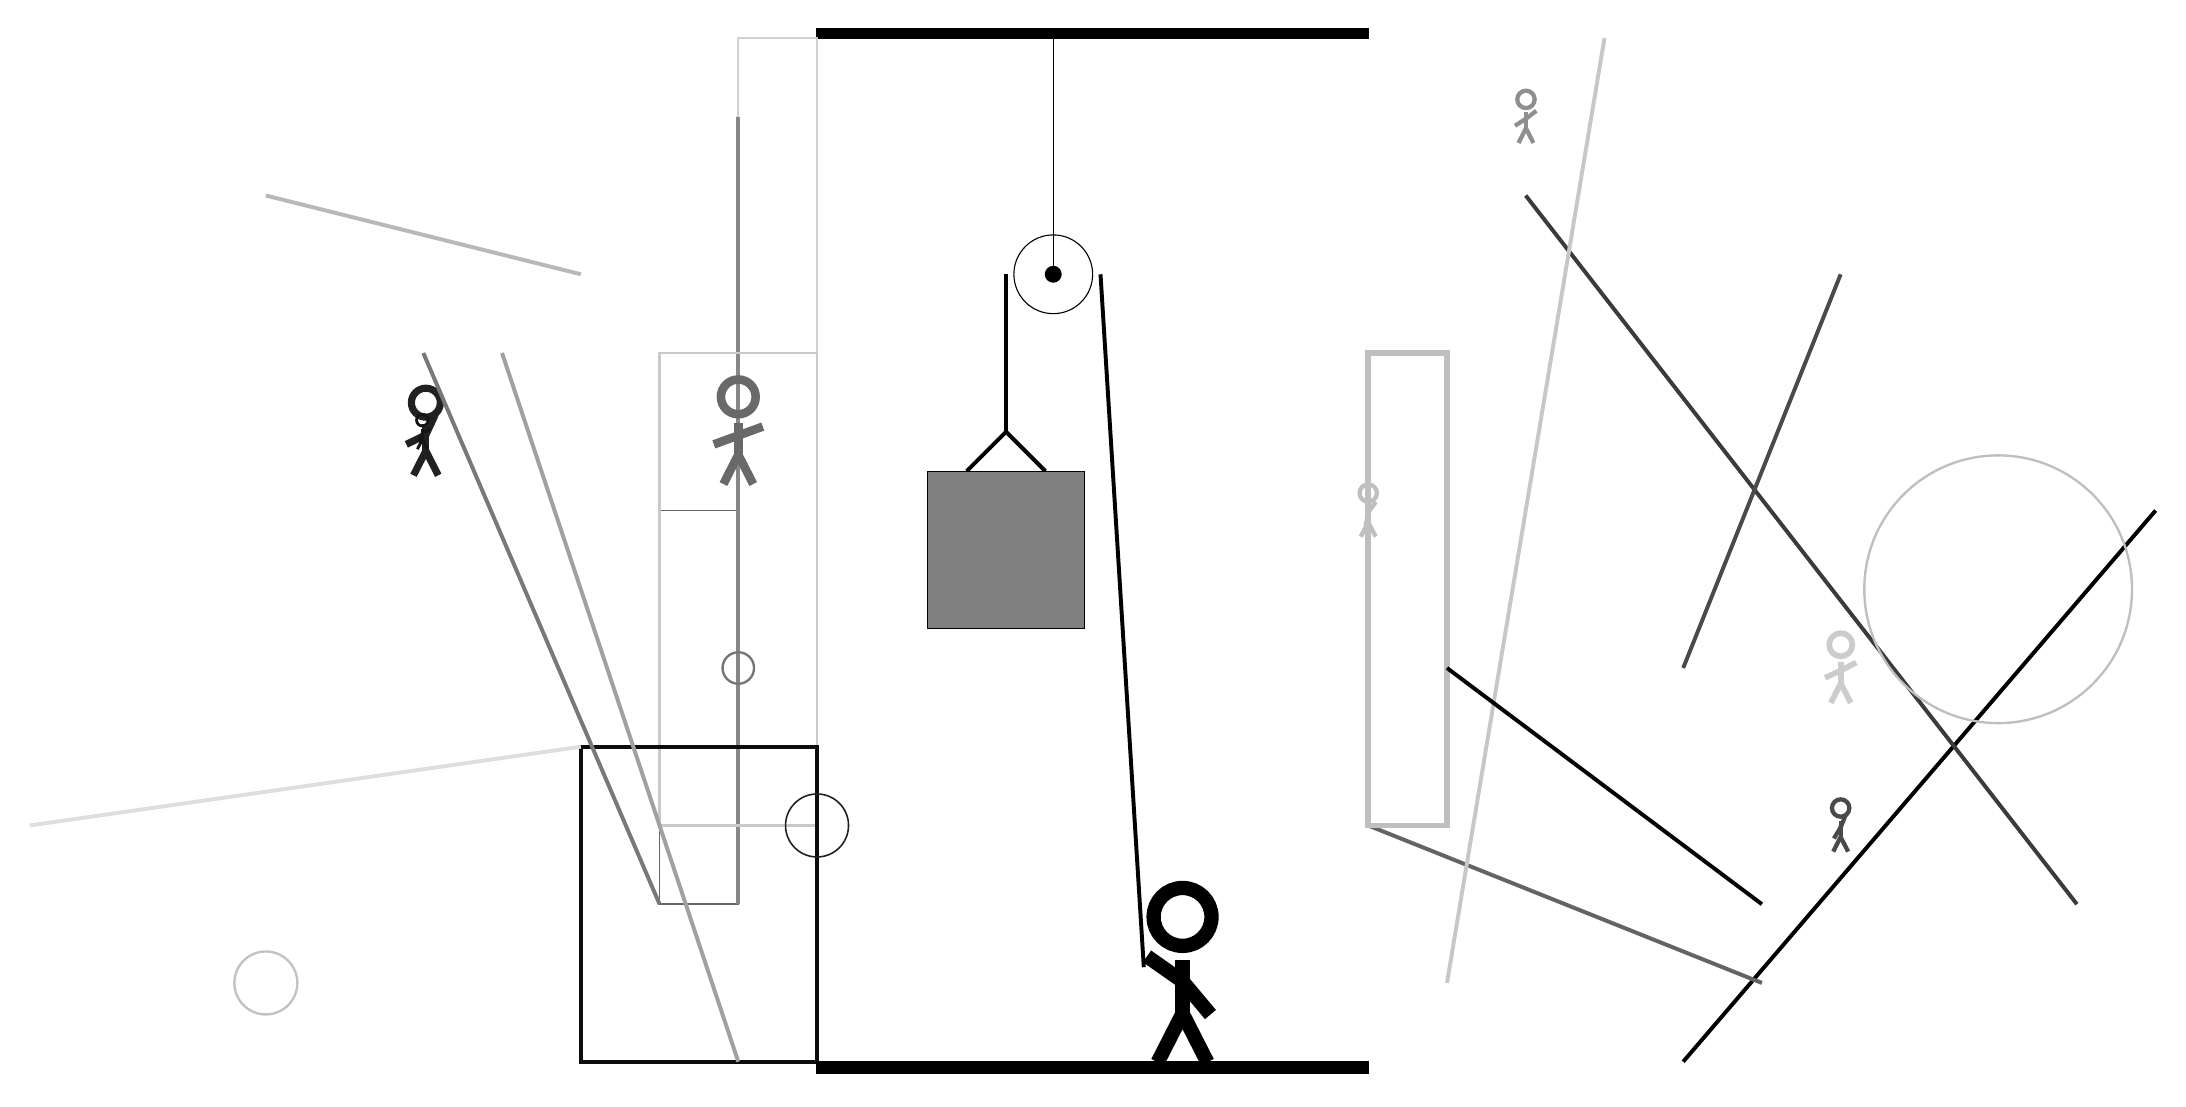
\begin{tikzpicture}
		%%%%% START %%%%%
		
		\draw[fill=black] (-2, 10) rectangle (5, 10.125);
		
		\draw (1, 7) circle (0.5);
		\draw[fill=black] (1, 7) circle (0.1);
		\draw (1, 10) -- (1, 7);
		
		\draw[line width=0.2mm, color=black!60] (-4, -1) rectangle (-3, 4);
		
		\draw[line width=0.3mm, color=black!18] (-3, 10) rectangle (-2, 6);
		\draw[line width=0.5mm, color=black!100](9, -3) -- (15, 4);
		\draw[line width=0.5mm, color=black!77](7, 8) -- (14, -1);
		
		\draw[line width=0.5mm, color=black!47] (-3, 9) rectangle (-3, -1);
		\draw[line width=0.5mm, color=black!61](10, -2) -- (5, 0);
		\draw[line width=0.3mm, color=black!21] (-4, 6) rectangle (-2, 0);
		
		\draw[line width=0.7mm, color=black!25] (6, 0) rectangle (5, 6);
		\draw[line width=0.5mm, color=black!95] (-2, 1) rectangle (-5, -3);
		\draw[line width=0.5mm, color=black!71](9, 2) -- (11, 7);
		
		\node[line width=0.6mm, color=black!59] at (-3, 5) {\Strichmaxerl[6][20][20]};
		\node[line width=0.2mm, color=black!44] at (7, 9) {\Strichmaxerl[3][33][37]};
		\draw[line width=0.5mm, color=black!13](-5, 1) -- (-12, 0);
		
		\node[line width=0.5mm, color=black!71] at (11, 0) {\Strichmaxerl[3][59][68]};
		\draw[line width=0.5mm, color=black!22](8, 10) -- (6, -2);
		\node[line width=0.6mm, color=black!87] at (-7, 5) {\Strichmaxerl[5][26][65]};
		
		\node[line width=0.4mm, color=black!20] at (11, 2) {\Strichmaxerl[4][25][27]};
		\draw[line width=0.5mm, color=black!99](6, 2) -- (10, -1);
		\draw[line width=0.5mm, color=black!37](-6, 6) -- (-3, -3);
		\draw [line width=0.2mm, color=black!88](-2, 0) circle (0.4);
		\draw [line width=0.3mm, color=black!54](-3, 2) circle (0.2);
		
		\draw [line width=0.3mm, color=black!24](-9, -2) circle (0.4);
		
		\draw[line width=0.5mm, color=black!28](-5, 7) -- (-9, 8);
		\draw [line width=0.5mm, color=black!72](8, 5) circle (0.0);
		\draw [line width=0.3mm, color=black!25](13, 3) circle (1.7);
		
		\draw[line width=0.5mm, color=black!53](-7, 6) -- (-4, -1);
		\node[line width=0.6mm, color=black!92] at (-7, 5) {\Strichmaxerl[2][63][27]};
		\node[line width=0.2mm, color=black!25] at (5, 4) {\Strichmaxerl[3][79][54]};
		
		\draw[line width=0.5mm] (-0.1, 4.5) -- (0.4, 5.0) -- (0.9, 4.5);
		\draw[fill=black!50] (-0.6, 4.5) rectangle (1.4, 2.5);
		
		\draw[line width=0.5mm] (0.4, 7) -- (0.4, 5.0);
		\centerarc[line width=0.5mm](1, 7)(0:180:0.6);
		\draw[line width=0.5mm](1.6, 7) -- (2.15, -1.8);
		
		\node at (2.6, -1.9) {\Strichmaxerl[10][-35][-50]};
		
		\draw[fill=black] (-2, -3) rectangle (5, -3.15);
		
		%%%%% END %%%%%
	\end{tikzpicture}
\end{document}